\section{Arduino vs. RaspberryPi} 

\begin{frame}
\frametitle{Worin unterscheiden sich die beiden Bastlerplatinen?} 
Auf den ersten Blick bietet der Raspberry Pi mehr als 1000 mal soviel Rechenleistung wie ein Arduino Uno f�r zehn Euro Aufpreis. Da f�llt die Entscheidung leicht, oder?

Sehen wir uns die Unterschiede doch einmal n�her an:
\end{frame}

\subsection{Technische Daten}
\begin{frame}
\frametitle{Speicher und Rechenleistung} 
\begin{tabular}{c c c c}
\textbf{Plattform} & \textbf{Arduino} & \textbf{Raspberry Pi} & \textbf{Faktor} \\ 
\pause 
RAM/Variablenspeicher & 2048 & 536870912 & 262144\\
\pause 
Festspeicher & 32768 & 8589934592 & 262144 \\
\pause
Wortbreite & 8Bit & 32Bit & 4 \\
\pause 
,,Rechenleistung'' (MIPS) &  16 & ~ 1000 & 64 \\
\end{tabular} 
\end{frame}

\begin{frame}
\frametitle{IO und Buses}
Arduino heisst in diesem Kontext Atmega328P, Raspberry Pi meint das Model B...
\newline

\begin{tabular}{c c c c}
\textbf{Plattform} & \textbf{Arduino} & \textbf{Raspberry Pi} & \textbf{Faktor} \\ 
\pause
GPIO digital & 17 & 8 & unfair! �pfel vs Birnen! \\
\pause
analog & 6 & 0 & 0 \\
\pause
SPI & 1 & 2 & 2 \\
\pause
UART (seriell) & 1 & 1 & 1 \\
\pause
I2C & 1 & 1 & 1 \\
\end{tabular} 
\end{frame}

\begin{frame}
\frametitle{Interrupts} 
Arduino heisst in diesem Kontext Atmega328P, Raspberry Pi meint das Model B...
\newline

\begin{tabular}{c c c c}

\textbf{Plattform} & \textbf{Arduino} & \textbf{Raspberry Pi} & \textbf{Faktor} \\ 
\pause
Steigend/Fallend & 2 & 8? Publikum? & ? \\
\pause
Wakeup-Timer & 2 & beliebig viele & ? \\
\end{tabular} 

\end{frame}

\begin{frame}
\frametitle{Leistungsaufnahme} 

Arduino heisst in diesem Kontext Atmega328P, Raspberry Pi meint das Model B...
\newline

\begin{tabular}{c c c c}

\textbf{Plattform} & \textbf{Arduino} & \textbf{Raspberry Pi} & \textbf{Faktor} \\ 
\pause
\textbf{ohne Optimierungen} & 40mA bei 5V & 300mA bei 5V & 7,5 \\
\pause
\textbf{optimiert} & 4$\mu$A bei 3,0V & 60mA bei 3,6V & 15000 \\
\pause
\end{tabular}

\begin{itemize}
\item Optimierungen beim Arduino: BOD abschalten, ADC abschalten, Tiefschlaf, Batteriebetrieb mit 2xAAA, Takt auf 8MHz reduziert.
\item Optimierungen beim Raspberry Pi: Abschalten nicht ben�tigter Schnittstellen, Aufl�ten eines optimierten Spannungswandlers, Akkubetrieb mit 3,6V.
\end{itemize}

\end{frame}

\begin{frame}
\frametitle{Preise} 
 
 Auf den ersten Blick liegen Arduino und Raspberry Pi preislich eng beieinander. Auf den zweiten Blick:
 
\begin{itemize}
\item Raspberry Pi: 35 bis 40 \euro
\pause
\item Arduino Uno oder Zero: 25 bis 30 \euro
\pause
\item Arduino Pro Mini (Sparkfun oder Watterott): 10 \euro
\pause
\item Arduino Pro Mini (China-Klon): 3 bis 4 \euro
\pause
\item Atmega328P im DIL28-Geh�use: 3 bis 5 \euro
\end{itemize}
\end{frame}

\begin{frame}
\frametitle{Preise visualisiert} 

Der Raspberry links war teurer als die Arduino-Klone und nackten Atmega328P rechts!

  \begin{center}
    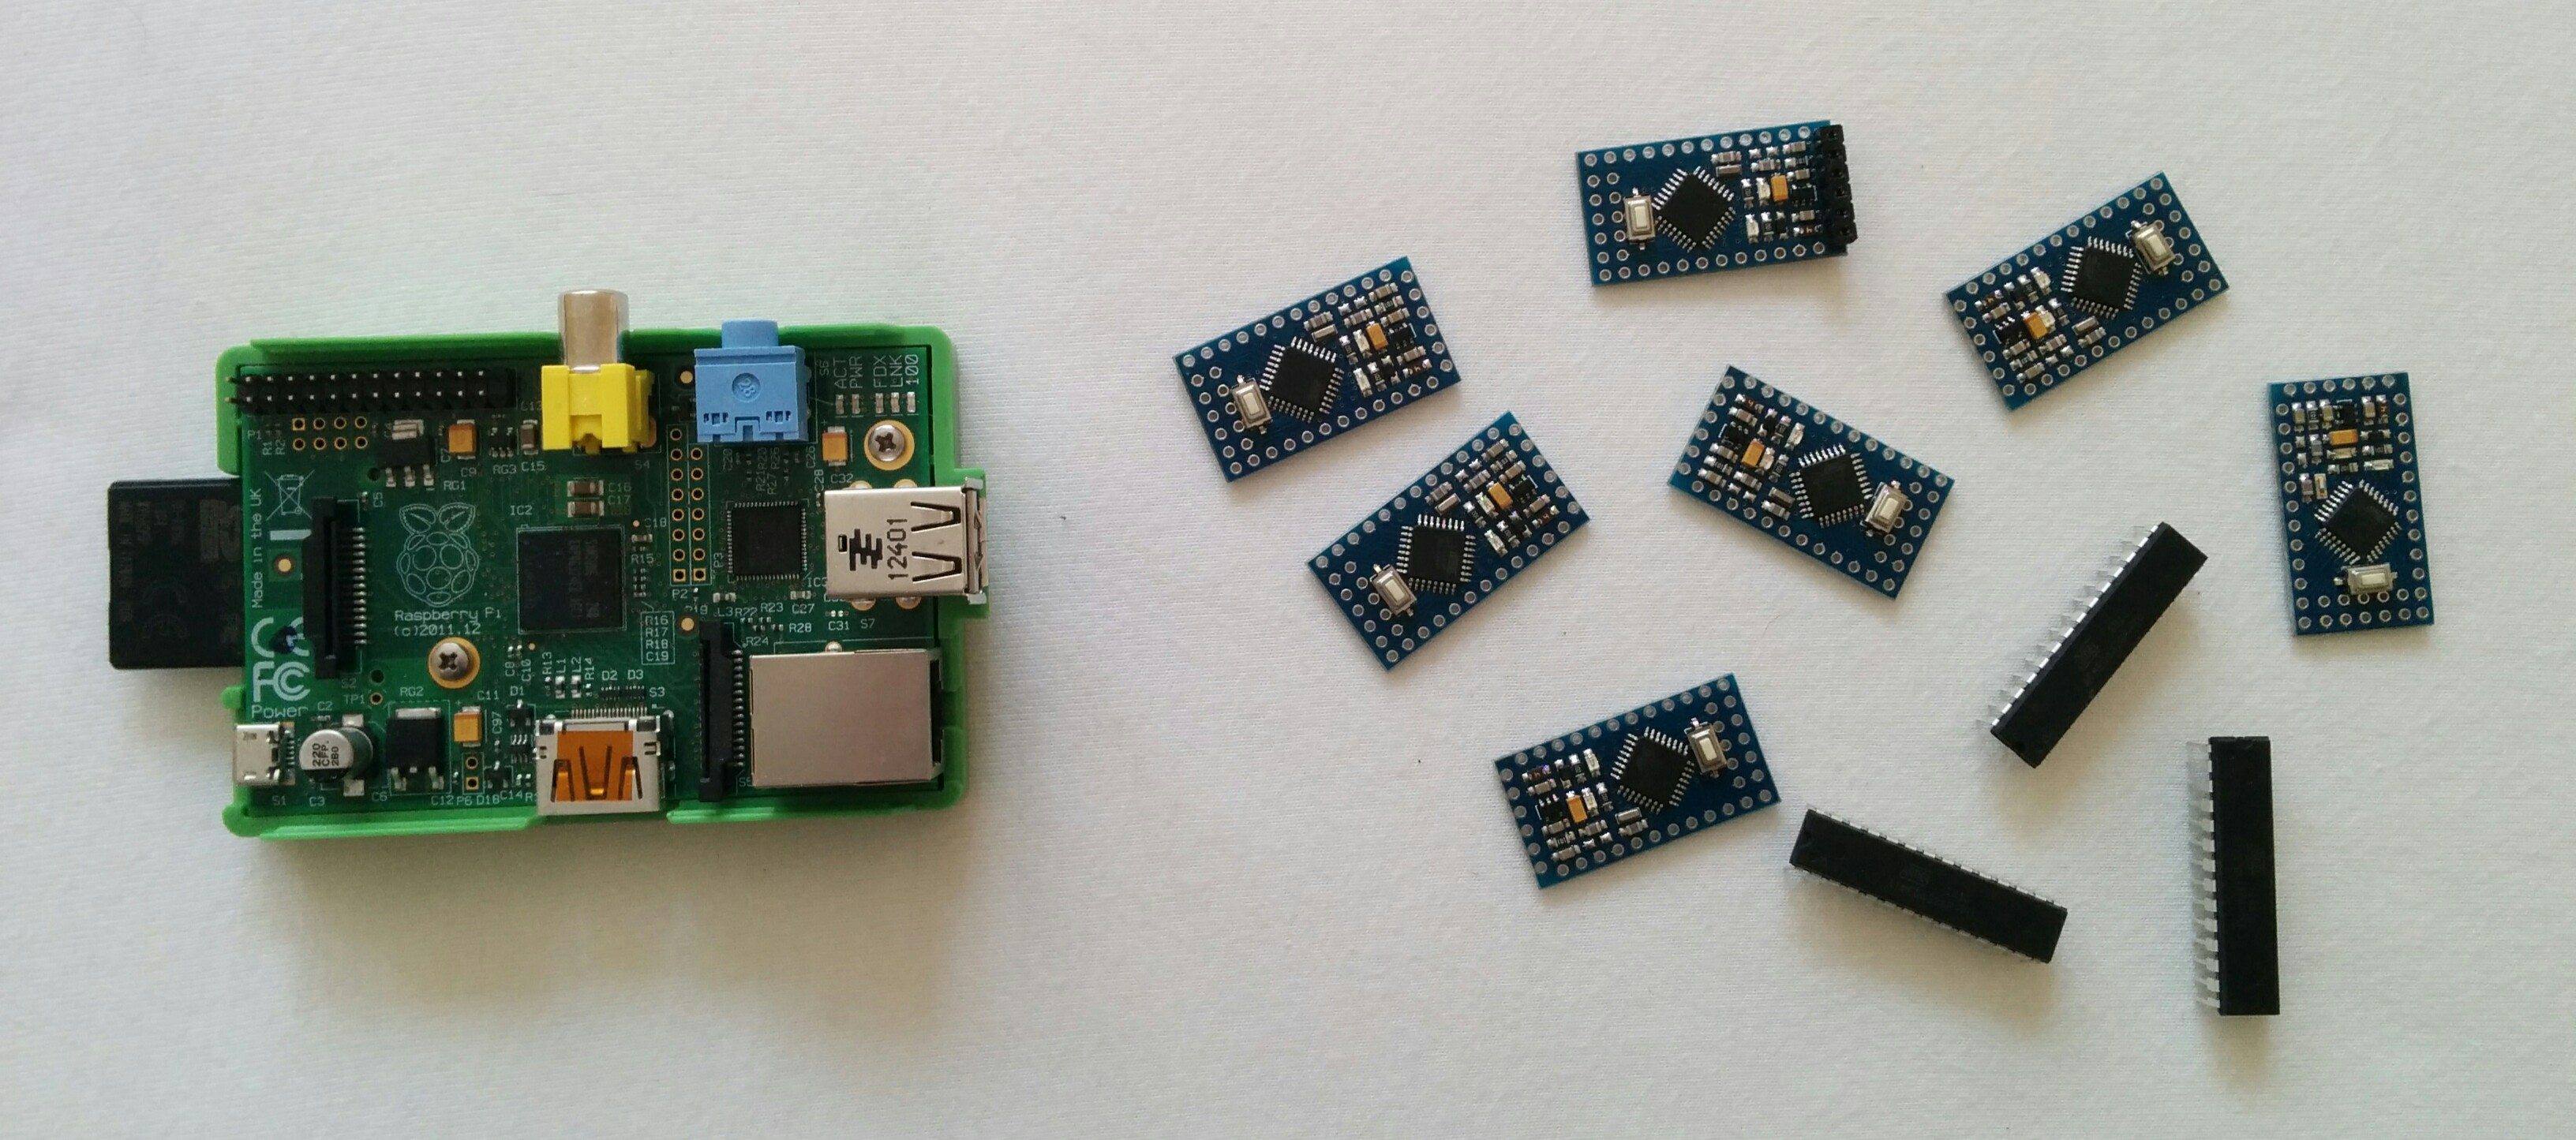
\includegraphics[width=10cm]{photos/IMG_20140626_101926.jpg}
  \end{center}
\end{frame}


\subsection{Einsatzbereiche}

\begin{frame}
\frametitle{Arduino} 
\begin{itemize}
\item \emph{Energiesparende} Sensoren oder Aktoren: Jahrelanger Betrieb auf zwei AAA-Zellen m�glich
\item \emph{Billige} Sensoren: Totalverlust ist zu verschmerzen
\item \emph{Billige} Peripherie: Der integrierte ADC erlaubt den Anschluss von Thermistoren statt One-Wire-Temperatursensoren
\item \emph{Einfache} Sensoren und Aktoren: auch gr��ere St�ckzahlen (Sensornetze, Kunstprojekte) lassen sich mit wenigen Bauteilen schnell fertigen
\item \emph{Robuste} Softwareentwicklung: Weit weniger Abstraktionsschichten, bessere Vorhersehbarkeit
\end{itemize}
\end{frame}


\begin{frame}
\frametitle{Temperatursensor mit Webserver} 

Der simpelste aller Webserver: Jedes auf Port 80 eingehende Paket - egal, was drinsteht -  wird einfach mit einer Webseite (Temperatur und Luftfeuchte) beantwortet. Weniger als 20k Bin�rcode gesamt!

\begin{itemize}
\item Arduino Pro Mini oder nackter Atmega328P
\item Enc28J60 Ethernet (SPI-Anbindung)
\item DHT11/22 Sensor
\item Gesamtkosten: ca. 12  \euro
\end{itemize}
\end{frame}

\begin{frame}
\frametitle{Temperatursensor mit Webserver} 

So sieht der verl�tete Aufbau aus:

  \begin{center}
    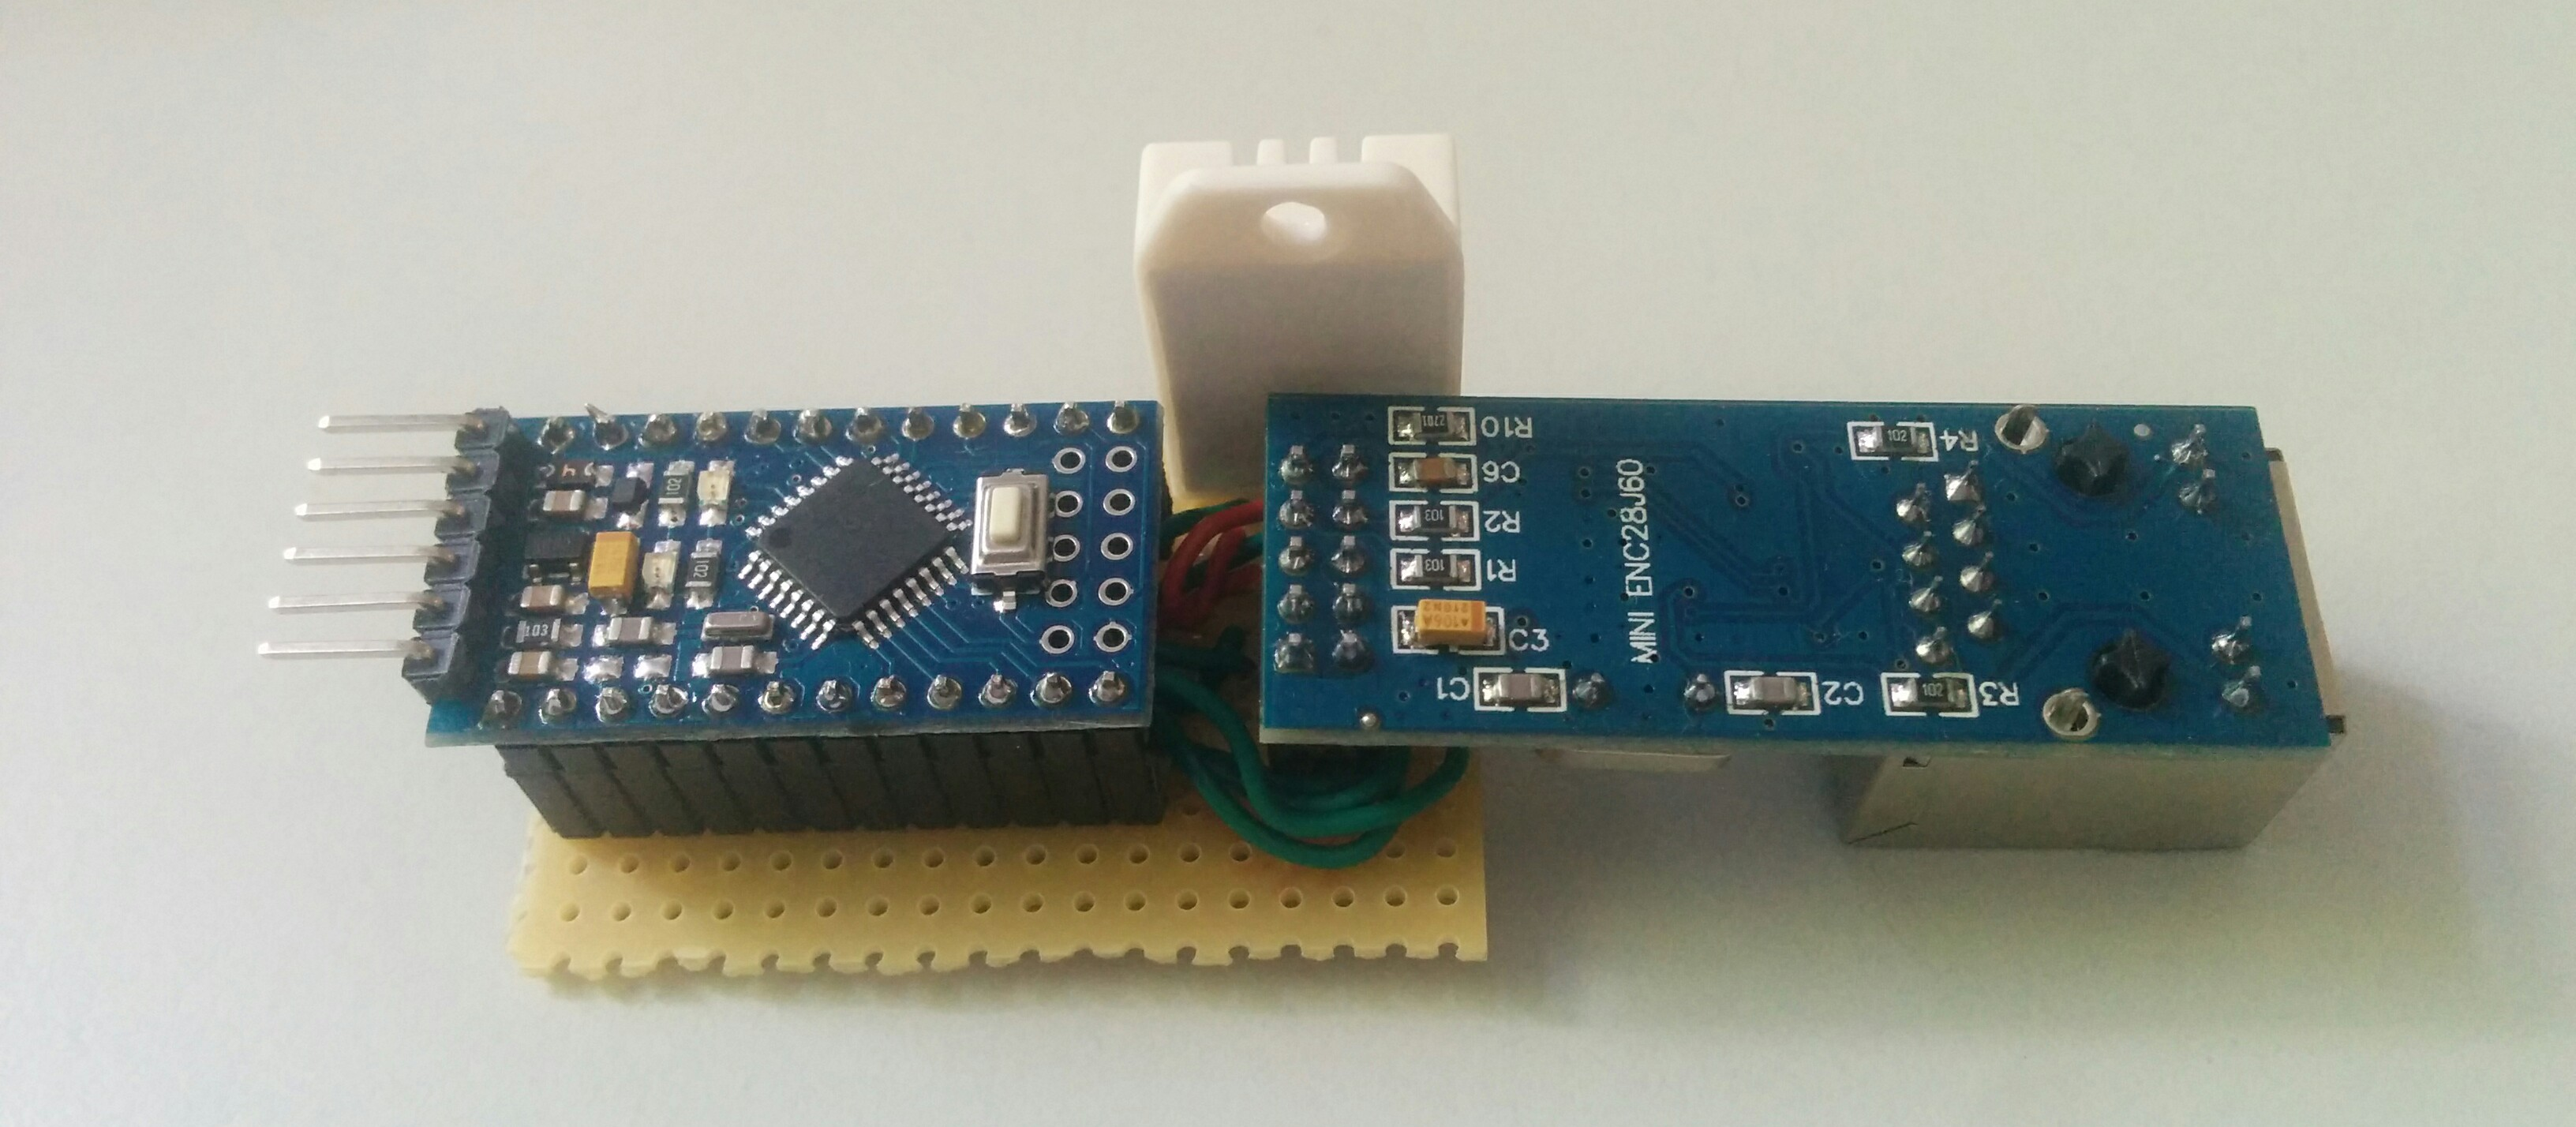
\includegraphics[width=10cm]{photos/IMG_20140626_105909.jpg}
  \end{center}
\end{frame}

\begin{frame}
\frametitle{Code auf https://github.com/mschlenker} 
 \begin{center}
    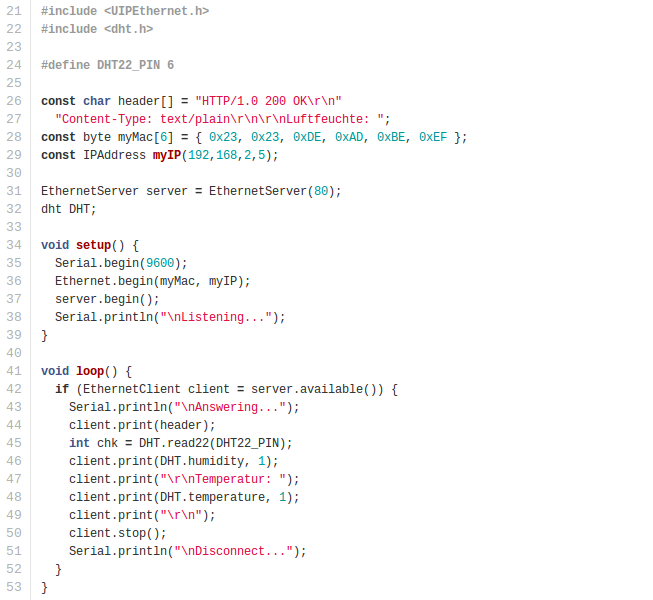
\includegraphics[width=7.5cm]{photos/codedhtserver.png}
  \end{center}
\end{frame}

\begin{frame}
\frametitle{Loggender Sensor (Temperatur, Erdfeuchte, Licht)} 
\begin{itemize}
\item Arduino Pro Mini oder nackter Atmega328P
\item $\mu$SD-Kartenadapter (geschenkt!)
\item diverse Analogsensoren (NTC, resistive Erdfeuchte, Photo-Widerstand...)
\item hier zus�tzlich: RTC
\item Gesamtkosten: 5 bis 10 Euro \euro
\item ca. ein Jahr Laufzeit auf 3xAA bei Optimierung
\end{itemize}
\end{frame}

\begin{frame}
\frametitle{Sensor mit SD-Logging} 

So sieht der verl�tete Aufbau aus:

  \begin{center}
    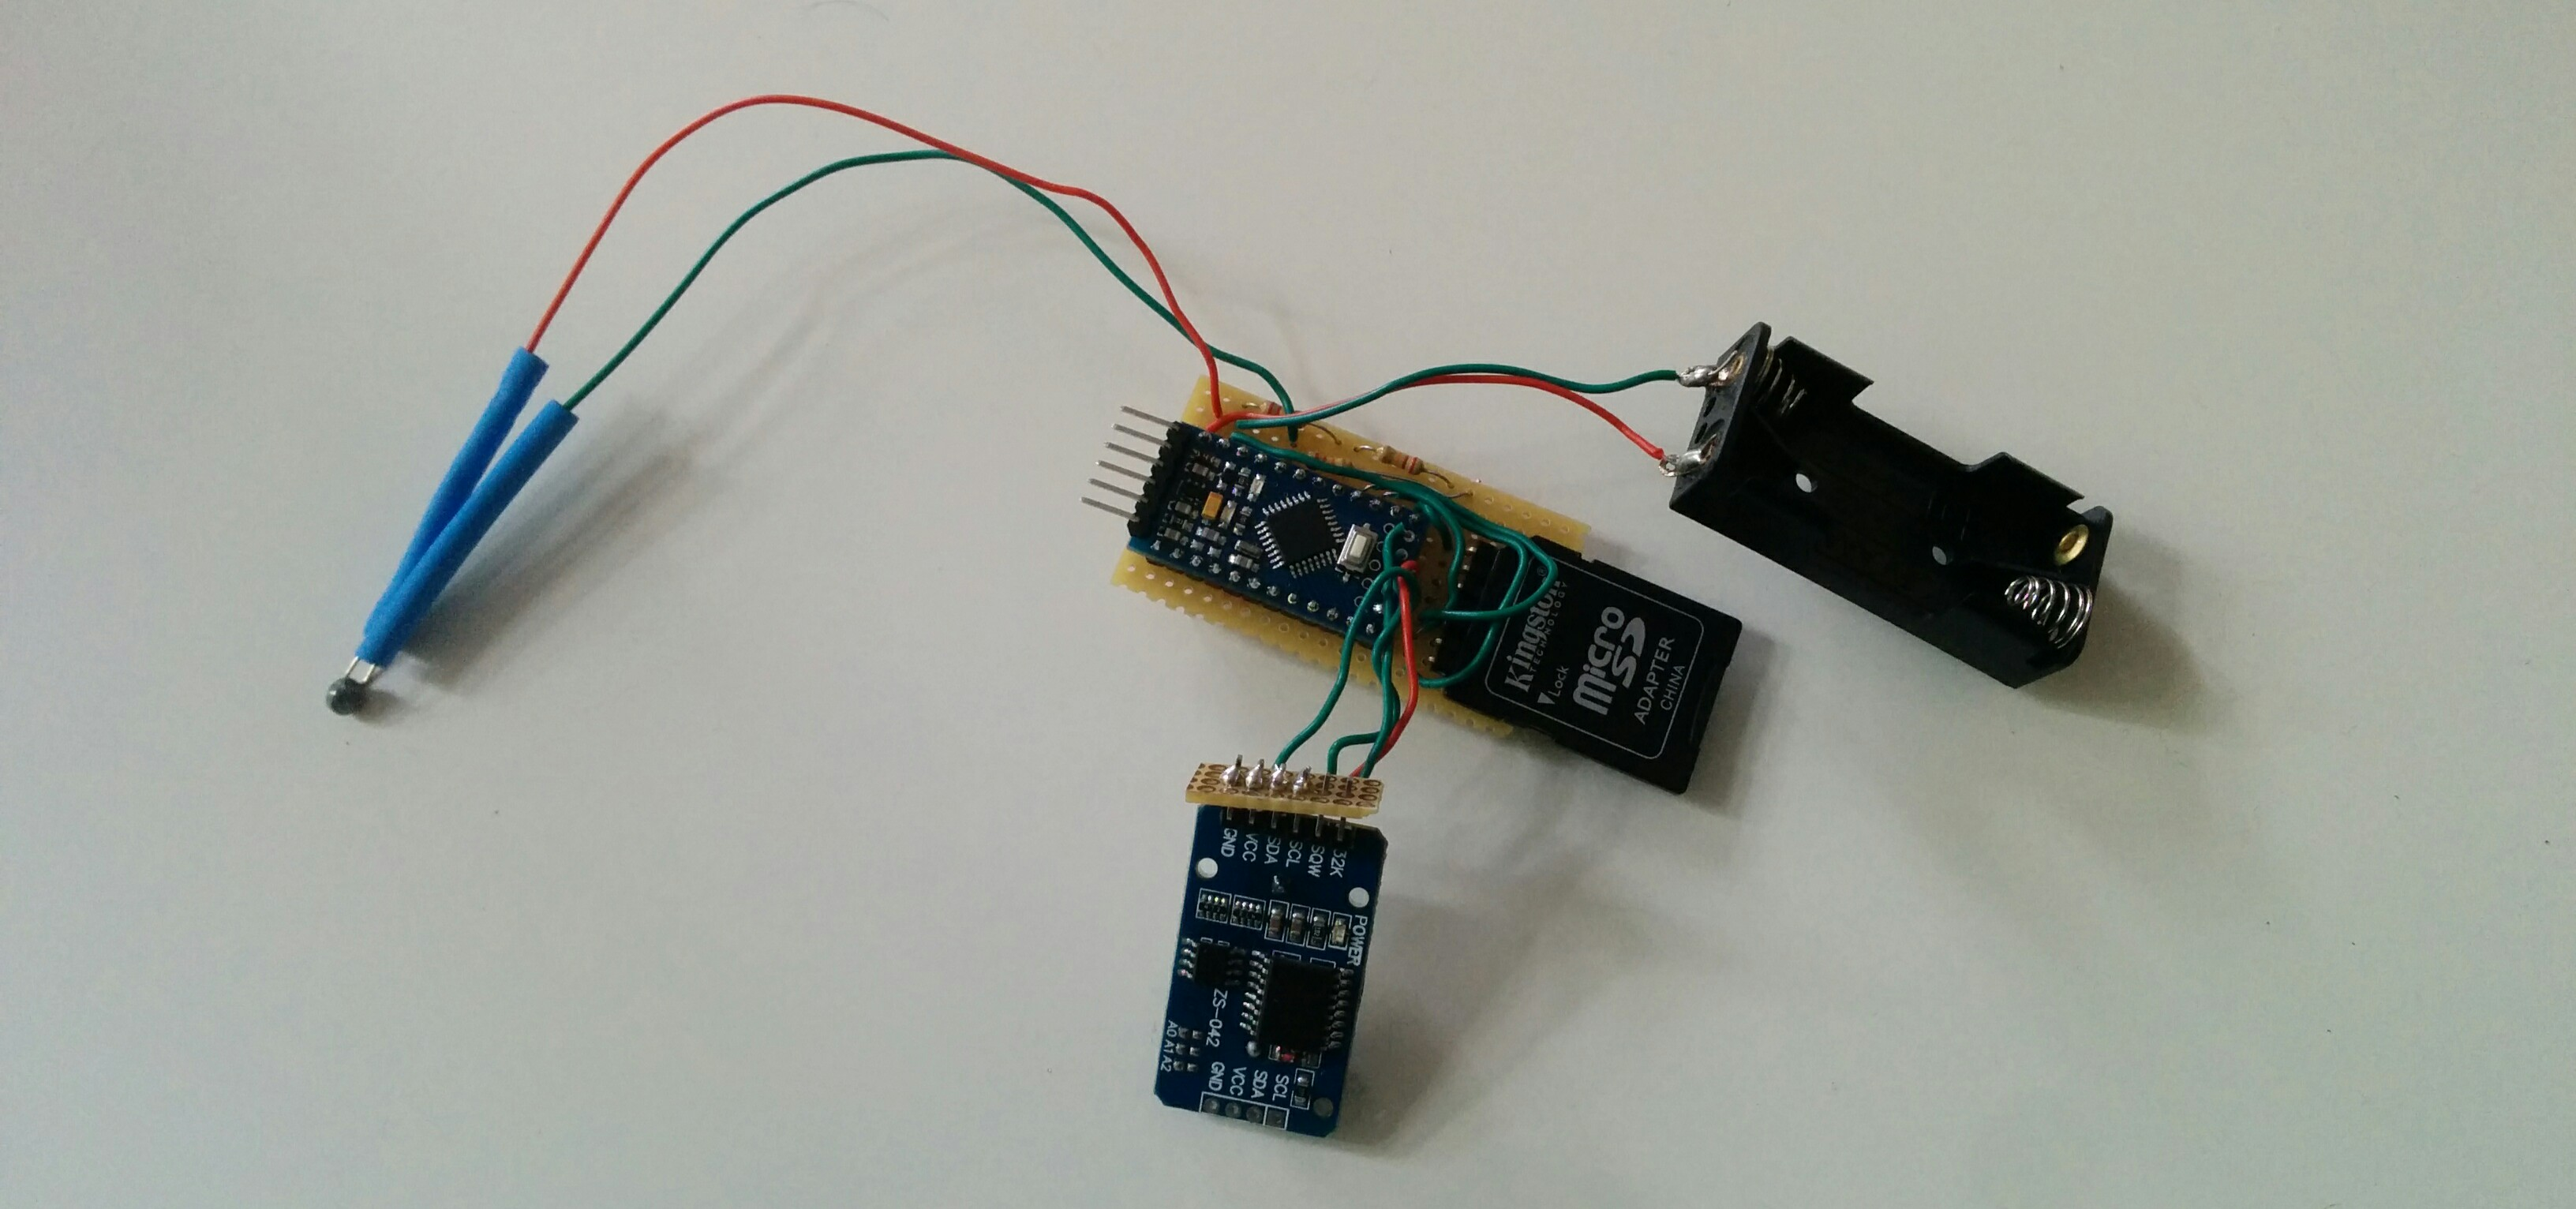
\includegraphics[width=10cm]{photos/IMG_20140626_111628.jpg}
  \end{center}
\end{frame}

\begin{frame}
\frametitle{Raspberry Pi} 
\begin{itemize}
\item \emph{Billige} Basis f�r Sensornetze
\item \emph{Stromsparende} ,,Au�enstelle'': Solarbetrieb mit relativ kleinem Panel m�glich
\item \emph{Gro�e} Flexibilit�t dank ,,normalem'' Linux
\item \emph{Kleine Server} f�r den Hausgebrauch
\item \emph{Stark genug} um bspw. DVB-T oder Webcam zu streamen
\item \emph{Lautloser} Thin Client f�r Windows- oder Linux-Server
\end{itemize}
\end{frame}

